\documentclass[journal,a4paper]{IEEEtran}

% Graphics
\usepackage{graphicx}

% Mathematics
\usepackage{amsmath}
\usepackage{amssymb}
\usepackage{amsthm}
\usepackage{mathtools}
\usepackage{bm}
\usepackage{tikz}
\usetikzlibrary{positioning,arrows.meta,shapes.symbols,shapes.geometric}

% Typography
\usepackage[T1]{fontenc}
\usepackage{microtype}

% References and links
\usepackage[hidelinks]{hyperref}
\usepackage[ backend=biber, style=ieee, doi=false, isbn=false, maxnames=3, minnames=2 ]{biblatex}
\addbibresource{references.bib}

\title{OMA in Senmos: Enabling a new level of analysis}
\author{Mark~Mizzi\\
Software Engineer, KI Monitoring\\
\texttt{mmi@ki.dk}}

\begin{document}

\maketitle

\begin{abstract}
    Operational Modal Analysis (OMA) is a powerful technique which allows engineers to model vibrations in complex man-made structures based on measurement data gathered from accelerometer arrays. In this work, we present our implementation of OMA in the Senmos monitoring platform as well as potential applications. Our main contribution is improved ease of use compared to traditional software solutions for OMA. We compare results obtained from our OMA implementation with the more traditional modeling technique of finite element analysis (FEM).
\end{abstract}

\section{Introduction}

Operational Modal Analysis (OMA) encompasses a set of techniques developed to compute and visualize modal vibrations of structures from real-world measurements. In this article we present an implementation of OMA built on the Senmos structural health monitoring (SHM) platform and its potential applications. 

Every structure has a set of natural frequencies which it tends to vibrate at when excited by an outside force. For instance, if a swing is lifted upwards and released, it swings back and forth at a rate determined by the length of its ropes. The same phenomenon occurs in more complex structures, but modeling natural frequencies from physical characteristics becomes significantly more complex. Furthermore, physical characteristics may change over time due to weathering, modifications, etc., requiring costly changes to such models. OMA algorithms address both of these issues by estimating natural frequencies from a window of measurement signals gathered at several points of the structure.

Each natural frequency $f_k$ also has an associated mode shape $\bm{\phi}_k$ which dictates the relative amplitude and phase (encoded as a complex number) at which each measurement point on a structure oscillates. The damping ratio $\zeta_k$ quantifies how quickly oscillation in a specific mode decays, relative to the natural frequency $f_k$. For instance, a damping ratio of $0.01$ indicates that after one oscillation, the amplitude has decreased by $0.01 \times 2\pi \approx 6.3\%$. OMA algorithms typically produce estimates of mode shapes and damping ratios in addition to natural frequencies.

% OMA algorithms are windowed algorithms; they produce results for a window of measurements with a specified length, typically chosen on the order of 30 minutes to a few hours.

Existing OMA implementations~\cite{pyoma2} are obtuse and require ad-hoc scripting to set up for specific projects. The resulting source code is often not applicable to another project, requiring a duplication of efforts for every new project. Furthermore, no functionality is provided to run OMA continuously on an incoming stream of measurement data. All of the above collude to render OMA inaccessible to non-experts and domain experts who may not be intimately familiar with computer programming. Our implementation addresses these issues by providing a user-friendly interface built on pyOMA v2~\cite{pyoma2}.

The remainder of this article is structured as follows: Section~\ref{sec:theory} discusses theoretical background. Section~\ref{sec:practical} discusses the high level organization of our OMA implementation and its practical applications in SHM. Section~\ref{sec:further} relates OMA to other modeling techniques. Section~\ref{sec:conclusion} gives concluding remarks.

\section{Theoretical Backgound}\label{sec:theory}

OMA techniques can be broadly classified into frequency-domain decomposition (FDD) methods, and stochastic subspace identification (SSI) methods.

\subsection{FDD-Based Methods}\label{sec:fdd}

FDD-based methods~\cite{Brincker2000OutputonlyMA,Brincker2001DampingEB} operate on a frequency domain representation of measurement signals, typically the power spectral density (PSD) matrix $\mathbf{G}_{yy}\left(\omega \right)$ which collects all cross-spectral power densities.

Under mild conditions, the input PSD matrix ${\mathbf{G}}_{\mathrm{xx}}\left(\omega \right)$ can be related to the output PSD matrix ${\mathbf{G}}_{yy}\left(\omega \right)$ (corresponding to the actual sensor measurements) by:
\[
\mathbf{G}_{yy}\left(\omega \right) = 
\mathbf{H}^{\dagger}\left(\omega \right)\mathbf{G}_{xx}\left(\omega \right)\mathbf{H}\left(\omega \right)
\]
where $\mathbf{H}(\omega)$ is the unknown Frequency Response Function (FRF) matrix determining the system-environment interaction.

At a given frequency $\omega$, only 1-2 modes contribute significantly to the system output. Assuming that external forces have a white noise spectrum~\cite{Brincker2000OutputonlyMA}, 
\begin{equation}
\bar{G}_{yy}(\omega)
=
\sum_{k}
\left(
\frac{d_k \bm{\phi}_k \bm{\phi}_k^{T}}{j\omega-\lambda_k}
+
\frac{\bar{d}_k \bar{\bm{\phi}}_k \bar{\bm{\phi}_k^{T}}}
{j\omega-\bar{\lambda}_k}
\right)
\label{eq:fsdd-decomp}
\end{equation}
where $\lambda_k = 2\pi f_k\left(-\zeta_k + j\right)$, $d_k$ is the relative contribution of each mode, and the sum is over \textit{significant} modes.

Supposing natural frequencies have clearly separable spectral peaks, Eq.~\eqref{eq:fsdd-decomp} implies that $\bar{G}_{yy}(\omega) \to \frac{d_k \bm{\phi}_k \bm{\phi}_k^{T}}{2\pi f_k\zeta_k}$ as $\omega \to 2\pi f_k$ where $f_k$ is a natural frequency. $\bm{\phi}_k$ will then correspond to the largest left singular vector of $\bar{G}_{yy}(\omega)$. Furthermore, since $\bar{G}_{yy}(\omega)$ is then $\approx$ rank-1, the corresponding singular value (SV) is much larger than the rest of the spectrum. By a similar analysis, one can show that if $k\ge 2$ natural frequencies have spectral peaks clustered around $f$, the corresponding mode shapes are proportional to the largest $k$ left singular vectors of $\bar{G}_{yy}(2\pi f)$ and the corresponding SVs dominate the spectrum.

FDD-based methods discretize the frequency spectrum, compute the singular-value decomposition (SVD) at each point, and then output a modal parameter estimation (MPE) plot depicting the largest $M$ singular values (normalized to the $[0,1]$ range) against the frequency $f$. The first and second scenarios highlighted above are clearly visible in such a plot as a peak reaching $\approx 1.0$ in the first SV and large peaks in the first $k$ SVs resp. Figure~\ref{fig:sv-plot} shows an example MPE plot produced by our implementation.

\begin{figure}
\centering
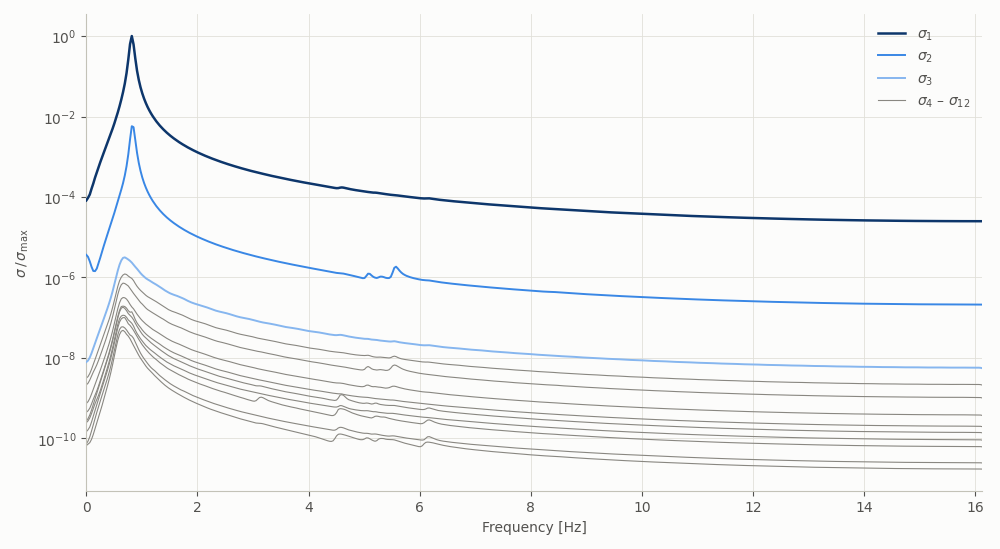
\includegraphics[width=\columnwidth]{figures/FDD-SV-plot-log.png}
\caption{
    MPE plot obtained from FSDD performed on a wind turbine. Note that the $y$-axis is plotted on a log-scale, which can help distinguish clustered modes from spurious peaks (noise). Measurements were collected from 4 accelerometers located at the base of the wind turbine tower, each measuring acceleration in three orthogonal directions. The plot shows an isolated peak in the largest SV around $0.8$, which is corroborated by a finite element model (FEM) of the tower that identified a natural frequency at $0.79$~\cite{PANDA2026124343}.
    }\label{fig:sv-plot}
\end{figure}

Once natural frequencies are selected, corresponding mode shapes can be obtained from the SVD, and damping ratios can be computed from the equations shown above.

Further improvements have been made to the basic scheme presented above such as frequency-spatial domain decomposition (FSDD)~\cite{fsdd} which we use in our implementation.

While precise and robust, FDD-based methods require manual selection of natural frequencies which can be time-consuming and requires expert identification for complicated scenarios, making it unsuitable for long-term, automatic analysis. We use FSDD as a one-time calibration step when a new project is configured, with the SSI-COV method (c.f. Section~\ref{sec:ssi}) used for long-term analysis.

\subsection{SSI-Based Methods}\label{sec:ssi}

SSI-based methods~\cite{ssi} model the (discrete-time) dynamics of the system using two linear equations:
\begin{align*}
    \mathbf{x}_{t+1} = \mathbf{A}\mathbf{x}_{t} + \mathbf{w}_t \\
    \mathbf{y}_{t+1} = \mathbf{C}\mathbf{x}_{t} + \mathbf{v}_t
\end{align*}
where $\mathbf{x}_t, \mathbf{y}_t$ are the system state and measurements collected at time $t$, while $\mathbf{w}_t, \mathbf{v}_t$ are random (white) noise signals caused by external forces and limited measurement precision resp.

It is convenient to collect $\{\mathbf{x}_{t}\}_{t=1}^T$ and $\{\mathbf{y}_{t}\}_{t=1}^T$ into $d\times T$ matrices $\mathbf{X}$ and $\mathbf{Y}$.

The SSI-COV algorithm is based on covariance matrices $\mathbf{R}_i$, defined for each row $\mathbf{y}^{(i)}$ of $\mathbf{Y}$ as:
\[
\mathbf{R}_i = \mathbf{y}^{(i)}\left(\mathbf{y}^{(i)}\right)^T
\]

It can be shown that
\[
\mathbf{R}_i = \mathbf{C}\mathbf{A}^{i-1}\mathbf{G}
\]
where $\mathbf{G} := \sum_{t=1}^{T-1}\mathbf{x}_{t+1}\mathbf{y}_t^T$. It follows that the block-Toeplitz matrix
\[
\mathbf{T}_{1|i} := \begin{pmatrix}
\mathbf{R}_i     & \mathbf{R}_{i-1} & \cdots & \mathbf{R}_1 \\
\mathbf{R}_{i+1} & \mathbf{R}_i     & \cdots & \mathbf{R}_2 \\
\vdots           & \vdots           & \ddots & \vdots       \\
\mathbf{R}_{2i-1}& \mathbf{R}_{2i-2}& \cdots & \mathbf{R}_i
\end{pmatrix}
\]
satisfies
\[
\mathbf{T}_{1|i} \;=\; \underbrace{
    \begin{pmatrix}
        \mathbf{C}\\
        \mathbf{C}\mathbf{A}\\
        \vdots\\
        \mathbf{C}\mathbf{A}^{i-1}
        \end{pmatrix}
        }_{\boldsymbol{\mathcal{O}}_i \,\in\, \mathbb{R}^{pq\times n}}\;\;\underbrace{\begin{pmatrix}\mathbf{A}^{i-1}\mathbf{G} & \mathbf{A}^{i-2}\mathbf{G} & \cdots & \mathbf{A}\mathbf{G} & \mathbf{G}\end{pmatrix}}_{\boldsymbol{\mathcal{C}}_i \,\in\, \mathbb{R}^{n\times pq}}
\]
where $n, p, q$ are the number of modes in the system, the dimensionality of the system state and the number of measurement channels resp.

The core idea of SSI-COV is to use SVD to decompose $\mathbf{T}_{1|i} \approx \mathbf{U}\mathbf{S}\mathbf{V}^T = (\mathbf{U}\mathbf{S}^{1/2})(\mathbf{S}^{1/2}\mathbf{V}^T)$ where the equality is approximate only the top $n$ singular values are kept, and $\mathbf{S}^{1/2}$ is the matrix obtained from $\mathbf{S}$ by taking $\sqrt{\cdot}$ of each element.

We then approximate $\mathcal{O}_i \approx \mathbf{U}\mathbf{S}^{1/2}$, which immediately yields an approximation of $\mathbf{C}$ (from the first block of $\mathcal{O}_i$) and a linear system which can be solved for $\mathbf{A}$ (by considering the relationship between blocks of $\mathcal{O}_i$).

Note that one prerequisite for applying SSI-COV is to know the number of modes $n$ in advance. Since this is usually an unknown, SSI-COV is typically computed for multiple values of $n$, and the most plausible $n$ is chosen using a stabilization diagram~\cite{Peeters01022000}.
We opt instead to use MPE plots from FSDD to allow the user to pick $n$ once during setup.

\section{Implementation}\label{sec:practical}

In this section we present our implementation of OMA, showcasing its ease of use and its application to structural health monitoring with a concrete example of a wind turbine project. Our work builds on the open source PyOMA2 package~\cite{pyoma2} by adding a user-friendly web interface which can be used by non-experts with minimal training. Figure~\ref{fig:impl-schematic} depicts the high level organization of our implementation.

\begin{figure}[t]
\centering
\resizebox{\columnwidth}{!}{%
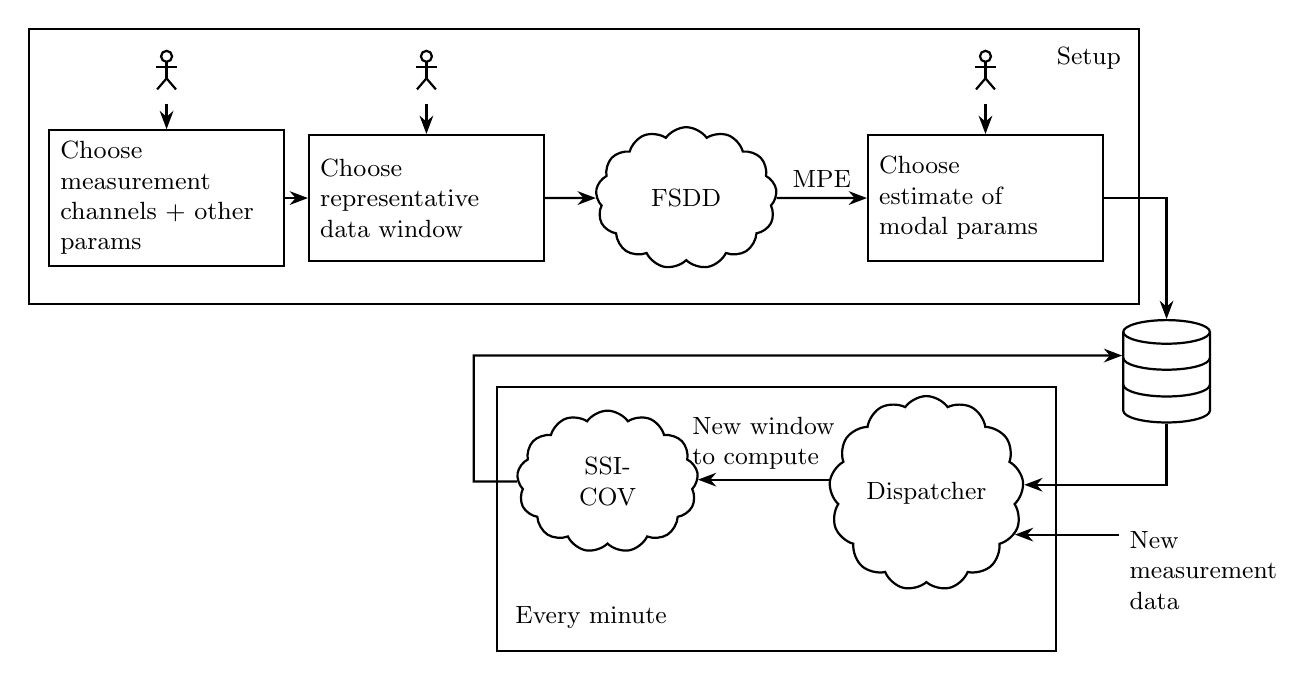
\begin{tikzpicture}[
    >=Stealth,
    line width=0.8pt,
    font=\small,
    box/.style={
        draw=black,
        align=left,
        text width=2.7cm,
        minimum height=1.6cm,
        inner sep=4pt,
        execute at begin node={\hyphenpenalty=10000}
    },
    proc/.style={
        cloud,
        draw=black,
        cloud puffs=13,
        cloud puff arc=110,
        align=center,
        inner sep=1pt,
        minimum width=2.3cm,
        minimum height=1.8cm
    },
    db/.style={
        inner sep=0pt,
        minimum width=1.1cm,
        minimum height=1.3cm
    },
    database/.pic={
        \draw (-0.55,0.5) -- (-0.55,-0.5) arc (180:360:0.55 and 0.15) -- (0.55,0.5);
        \draw (0,0.5) ellipse (0.55 and 0.15);
        \draw (-0.55,0.17) arc (180:360:0.55 and 0.15);
        \draw (-0.55,-0.17) arc (180:360:0.55 and 0.15);
    },
    actor/.pic={
        \draw (0,0.3) circle (0.07);
        \draw (0,0.23) -- (0,0.02);
        \draw (-0.13,0.16) -- (0.13,0.16);
        \draw (0,0.02) -- (-0.12,-0.12);
        \draw (0,0.02) -- (0.12,-0.12);
    }
]

% ---------------- Setup ----------------
\draw (0.55,7.6) rectangle (14.65,11.1);
\node[anchor=north east] at (14.55,11.0) {Setup};

% Users
\pic at (2.3,10.45) {actor};
\pic at (5.6,10.45) {actor};
\pic at (12.7,10.45) {actor};

% Setup steps
\node[box] (channels) at (2.3,8.95)
    {Choose measurement channels + other params};
\node[box] (window) at (5.6,8.95)
    {Choose representative data window};
\node[proc] (fsdd) at (8.9,8.95) {FSDD};
\node[box] (estimate) at (12.7,8.95)
    {Choose\\estimate of\\modal params};

\draw[->] (2.3,10.15) -- (channels.north);
\draw[->] (5.6,10.15) -- (window.north);
\draw[->] (12.7,10.15) -- (estimate.north);

\draw[->] (channels.east) -- (window.west);
\draw[->] (window.east) -- (fsdd.west);
\draw[->] (fsdd.east) -- node[above] {MPE} (estimate.west);

% ---------------- Database ----------------
\node[db] (db) at (15.0,6.75) {};
\pic at (db.center) {database};

\draw[->] (estimate.east) -| (db.north);

% ---------------- Every minute ----------------
\draw (6.5,3.2) rectangle (13.6,6.55);
\node[anchor=south west] at (6.6,3.35) {Every minute};

\node[proc] (ssi) at (7.9,5.35) {SSI-\\COV};
\node[proc] (disp) at (11.95,5.2) {Dispatcher};

\draw[->] (disp.172) -- node[above, align=left] {New window\\to compute} (ssi.east |- disp.172);

% SSI-COV results stored in database
\draw[->] (ssi.west) -- (6.2,5.35) |- (db.west |- 0,6.95);

% Database feeds dispatcher
\draw[->] (db.south) |- (disp.5);

% New measurement data
\node[align=left, anchor=north west] (newdata) at (14.4,4.85)
    {New\\measurement\\data};
\draw[->] (newdata.north west |- disp.-25) -- (disp.-25);

\end{tikzpicture}%
}
\caption{High level schematic overview of our OMA implementation.}\label{fig:impl-schematic}
\end{figure}


Key abstractions from Senmos such as sensor channels and sensors (groups of channels) are reused in the context of OMA; each frequency and damping mode is mapped to a sensor channel, and the user is given an option of automatically creating all required channels under a new sensor object. Reusing these abstractions automatically allows the user to apply signal processing algorithms available in Senmos to OMA outputs directly, as well as plot them.

Senmos aggregates data from a large number of heterogenous sources. In practice this means that measurement data often arrives out of order, with a time-varying delay, or not at all. Several complications requiring non-trivial design decisions arise due to the need to handle these issues; all of these are handled by our dispatcher implementation. The database tracks a marker with the end date of the last window processed for each OMA configuration. When the dispatcher runs a new refresh cycle, it calculates which OMA configurations may have new windows to process based on this marker and the window size/boundary configured by the user. Next, candidate windows are handed to a worker pool for processing. The number of candidate windows dispatched per configuration is limited to the last $N$ windows where $N$ is set to a suitable value. The assigned worker collects all measurement data falling inside the window and performs SSI-COV (c.f. Section~\ref{sec:ssi}) on it, aborting if the fill factor is below 10\%.

Since there is no reliable way to distinguish between a period of missing data and a large delay in sending data, the dispatcher also resets the marker of configurations which have fallen behind by more than $M$ days to a more recent date, so that such configurations catch up. A system administrator can manually recompute historical windows which have been skipped due to this design.

We see two potential applications for our OMA implementation:
\begin{enumerate}
    \item Sudden changes in natural frequencies predicted by OMA are a robust indicator of structural damage. % TODO CITE
    Given that Senmos features the ability to set range-based alarms, we see this as a valuable application of our implementation to SHM.
    Furthermore, alarms are easy for non-experts to configure and understand, making our solution uniquely appealing for this use case.

    \item Another, more fundamental application is the use of OMA to model and visualize vibrations on the structure. % TODO Flesh this out, explain dashboard feature

\end{enumerate}

\section{OMA vs. other modeling techniques}\label{sec:further}

% Compare to weaker techniques like peak picking, why do we need OMA?
% Compare to FEM. How precisely does it match FEM for our example?
% Argue how FEM can complement it
% How to convert results of OMA to stresses on the structure, with an easy UI 

\section{Conclusion}\label{sec:conclusion}

\printbibliography

\end{document}